%% abtex2-modelo-trabalho-academico.tex, v-1.9.7 laurocesar
%% Copyright 2012-2018 by abnTeX2 group at http://www.abntex.net.br/ 
%%
%% This work may be distributed and/or modified under the
%% conditions of the LaTeX Project Public License, either version 1.3
%% of this license or (at your option) any later version.
%% The latest version of this license is in
%%   http://www.latex-project.org/lppl.txt
%% and version 1.3 or later is part of all distributions of LaTeX
%% version 2005/12/01 or later.
%%
%% This work has the LPPL maintenance status `maintained'.
%% 
%% The Current Maintainer of this work is the abnTeX2 team, led
%% by Lauro César Araujo. Further information are available on 
%% http://www.abntex.net.br/
%%
%% This work consists of the files abntex2-modelo-trabalho-academico.tex,
%% abntex2-modelo-include-comandos and abntex2-modelo-references.bib
%%

% ------------------------------------------------------------------------
% ------------------------------------------------------------------------
% abnTeX2: Modelo de Trabalho Academico (tese de doutorado, dissertacao de
% mestrado e trabalhos monograficos em geral) em conformidade com 
% ABNT NBR 14724:2011: Informacao e documentacao - Trabalhos academicos -
% Apresentacao
% ------------------------------------------------------------------------
% ------------------------------------------------------------------------

\documentclass[
	% -- opções da classe memoir --
	12pt,				% tamanho da fonte
	%openright,			% capítulos começam em pág ímpar (insere página vazia caso preciso)
	%twoside,			% para impressão em recto e verso. Oposto a oneside
	oneside,
	a4paper,			% tamanho do papel. 
	% -- opções da classe abntex2 --
	%chapter=TITLE,		% títulos de capítulos convertidos em letras maiúsculas
	%section=TITLE,		% títulos de seções convertidos em letras maiúsculas
	%subsection=TITLE,	% títulos de subseções convertidos em letras maiúsculas
	%subsubsection=TITLE,% títulos de subsubseções convertidos em letras maiúsculas
	% -- opções do pacote babel --
	english,			% idioma adicional para hifenização
	french,				% idioma adicional para hifenização
	spanish,			% idioma adicional para hifenização
	brazil				% o último idioma é o principal do documento
	]{abntex2}

% ---
% Pacotes básicos 
% ---
\usepackage{lmodern}			% Usa a fonte Latin Modern			
\usepackage[T1]{fontenc}		% Selecao de codigos de fonte.
\usepackage[utf8]{inputenc}		% Codificacao do documento (conversão automática dos acentos)
\usepackage{indentfirst}		% Indenta o primeiro parágrafo de cada seção.
\usepackage{color}				% Controle das cores
\usepackage{graphicx}			% Inclusão de gráficos
\usepackage{microtype} 			% para melhorias de justificação
% ---
		
% ---
% Pacotes adicionais, usados apenas no âmbito do Modelo Canônico do abnteX2
% ---
\usepackage{lipsum}				% para geração de dummy text
% ---

% ---
% Pacotes de citações
% ---

\usepackage[
	backend=biber, style=abnt,  ittitles
]{biblatex}
\addbibresource{tcc.bib} % Seus arquivos de bibliografia vão aqui.

% Obsolete
%\usepackage[brazilian,hyperpageref]{backref}	 % Paginas com as citações na bibl
%\usepackage[alf]{abntex2cite}	% Citações padrão ABNT

% --- 
% CONFIGURAÇÕES DE PACOTES
% --- 

% ---
% Configurações do pacote backref
% Usado sem a opção hyperpageref de backref
%\renewcommand{\backrefpagesname}{Citado na(s) página(s):~}
%% Texto padrão antes do número das páginas
%\renewcommand{\backref}{}
%% Define os textos da citação
%\renewcommand*{\backrefalt}[4]{
%	\ifcase #1 %
%		Nenhuma citação no texto.%
%	\or
%		Citado na página #2.%
%	\else
%		Citado #1 vezes nas páginas #2.%
%	\fi}%
% ---

% ---
% Informações de dados para CAPA e FOLHA DE ROSTO
% ---
\titulo{Desenvolvimento de um \emph{chatbot} que simule interações humanas para tirar dúvidas de universitários}
\autor{Beatriz Paiva Alves e Lucas Breur}
\local{São Paulo - Brasil}
\data{2021}
\orientador{Prof. M.e Thiago Ribeiro Claro}
% \coorientador{Prof. M.Sc. Rodrigo Assirati Dias}
\instituicao{
  Centro Universitário Senac - Santo Amaro
 }
\tipotrabalho{Monografia}
% O preambulo deve conter o tipo do trabalho, o objetivo, 
% o nome da instituição e a área de concentração 
\preambulo{Monografia apresentada na disciplina Trabalho de Conclusão de Curso, como parte dos requisitos para obtenção do título de Bacharel em Ciência da Computação.}
% ---


% ---
% Configurações de aparência do PDF final

% alterando o aspecto da cor azul
\definecolor{blue}{RGB}{41,5,195}

% informações do PDF
\makeatletter
\hypersetup{
     	%pagebackref=true,
		pdftitle={\@title}, 
		pdfauthor={\@author},
    	pdfsubject={\imprimirpreambulo},
	    pdfcreator={LaTeX with abnTeX2},
		pdfkeywords={abnt}{latex}{abntex}{abntex2}{trabalho acadêmico}, 
		colorlinks=true,       		% false: boxed links; true: colored links
    	linkcolor=blue,          	% color of internal links
    	citecolor=blue,        		% color of links to bibliography
    	filecolor=magenta,      		% color of file links
		urlcolor=blue,
		bookmarksdepth=4
}
\makeatother
% --- 

% ---
% Posiciona figuras e tabelas no topo da página quando adicionadas sozinhas
% em um página em branco. Ver https://github.com/abntex/abntex2/issues/170
\makeatletter
\setlength{\@fptop}{5pt} % Set distance from top of page to first float
\makeatother
% ---

% ---
% Possibilita criação de Quadros e Lista de quadros.
% Ver https://github.com/abntex/abntex2/issues/176
%
\newcommand{\quadroname}{Quadro}
\newcommand{\listofquadrosname}{Lista de quadros}

\newfloat[chapter]{quadro}{loq}{\quadroname}
\newlistof{listofquadros}{loq}{\listofquadrosname}
\newlistentry{quadro}{loq}{0}

% configurações para atender às regras da ABNT
\setfloatadjustment{quadro}{\centering}
\counterwithout{quadro}{chapter}
\renewcommand{\cftquadroname}{\quadroname\space} 
\renewcommand*{\cftquadroaftersnum}{\hfill--\hfill}

\setfloatlocations{quadro}{hbtp} % Ver https://github.com/abntex/abntex2/issues/176
% ---

% --- 
% Espaçamentos entre linhas e parágrafos 
% --- 

% O tamanho do parágrafo é dado por:
\setlength{\parindent}{1.3cm}

% Controle do espaçamento entre um parágrafo e outro:
\setlength{\parskip}{0.2cm}  % tente também \onelineskip

% ---
% compila o indice
% ---
\makeindex
% ---

% ----
% Início do documento
% ----
\begin{document}

% Seleciona o idioma do documento (conforme pacotes do babel)
%\selectlanguage{english}
\selectlanguage{brazil}

% Retira espaço extra obsoleto entre as frases.
\frenchspacing 

% ----------------------------------------------------------
% ELEMENTOS PRÉ-TEXTUAIS
% ----------------------------------------------------------
% \pretextual

% ---
% Capa
% ---
\imprimircapa
% ---

% ---
% Folha de rosto
% (o * indica que haverá a ficha bibliográfica)
% ---
\imprimirfolhaderosto*
% ---

% ---
% Inserir a ficha bibliografica
% ---

% Isto é um exemplo de Ficha Catalográfica, ou ``Dados internacionais de
% catalogação-na-publicação''. Você pode utilizar este modelo como referência. 
% Porém, provavelmente a biblioteca da sua universidade lhe fornecerá um PDF
% com a ficha catalográfica definitiva após a defesa do trabalho. Quando estiver
% com o documento, salve-o como PDF no diretório do seu projeto e substitua todo
% o conteúdo de implementação deste arquivo pelo comando abaixo:
%
% \begin{fichacatalografica}
%     \includepdf{fig_ficha_catalografica.pdf}
% \end{fichacatalografica}

%\begin{fichacatalografica}
%	\sffamily
%	\vspace*{\fill}					% Posição vertical
%	\begin{center}					% Minipage Centralizado
%	\fbox{\begin{minipage}[c][8cm]{13.5cm}		% Largura
%	\small
%	\imprimirautor
%	%Sobrenome, Nome do autor
%	
%	\hspace{0.5cm} \imprimirtitulo  / \imprimirautor. --
%	\imprimirlocal, \imprimirdata-
%	
%	\hspace{0.5cm} \thelastpage p. : il. (algumas color.) ; 30 cm.\\
%	
%	\hspace{0.5cm} \imprimirorientadorRotulo~\imprimirorientador\\
%	
%	\hspace{0.5cm}
%	\parbox[t]{\textwidth}{\imprimirtipotrabalho~--~\imprimirinstituicao,
%	\imprimirdata.}\\
%	
%	\hspace{0.5cm}
%		1. Palavra-chave1.
%		2. Palavra-chave2.
%		2. Palavra-chave3.
%		I. Orientador.
%		II. Universidade xxx.
%		III. Faculdade de xxx.
%		IV. Título 			
%	\end{minipage}}
%	\end{center}
%\end{fichacatalografica}
% ---

% ---
% Inserir errata
% ---
%\begin{errata}
%Elemento opcional da \citeonline[4.2.1.2]{NBR14724:2011}. Exemplo:
%
%\vspace{\onelineskip}
%
%FERRIGNO, C. R. A. \textbf{Tratamento de neoplasias ósseas apendiculares com
%reimplantação de enxerto ósseo autólogo autoclavado associado ao plasma
%rico em plaquetas}: estudo crítico na cirurgia de preservação de membro em
%cães. 2011. 128 f. Tese (Livre-Docência) - Faculdade de Medicina Veterinária e
%Zootecnia, Universidade de São Paulo, São Paulo, 2011.

%\begin{table}[htb]
%\center
%\footnotesize
%\begin{tabular}{|p{1.4cm}|p{1cm}|p{3cm}|p{3cm}|}
%  \hline
%   \textbf{Folha} & \textbf{Linha}  & \textbf{Onde se lê}  & \textbf{Leia-se}  \\
%    \hline
%    1 & 10 & auto-conclavo & autoconclavo\\
%   \hline
%\end{tabular}
%\end{table}
%
%\end{errata}
% ---

% ---
% Inserir folha de aprovação
% ---

% Isto é um exemplo de Folha de aprovação, elemento obrigatório da NBR
% 14724/2011 (seção 4.2.1.3). Você pode utilizar este modelo até a aprovação
% do trabalho. Após isso, substitua todo o conteúdo deste arquivo por uma
% imagem da página assinada pela banca com o comando abaixo:
%
% \begin{folhadeaprovacao}
% \includepdf{folhadeaprovacao_final.pdf}
% \end{folhadeaprovacao}
%
%\begin{folhadeaprovacao}
%
%  \begin{center}
%    {\ABNTEXchapterfont\large\imprimirautor}
%
%    \vspace*{\fill}\vspace*{\fill}
%    \begin{center}
%      \ABNTEXchapterfont\bfseries\Large\imprimirtitulo
%    \end{center}
%    \vspace*{\fill}
%    
%    \hspace{.45\textwidth}
%    \begin{minipage}{.5\textwidth}
%        \imprimirpreambulo
%    \end{minipage}%
%    \vspace*{\fill}
%   \end{center}
%        
%   Trabalho aprovado. \imprimirlocal, 24 de novembro de 2012:
%
%   \assinatura{\textbf{\imprimirorientador} \\ Orientador} 
%   \assinatura{\textbf{Professor} \\ Convidado 1}
%   \assinatura{\textbf{Professor} \\ Convidado 2}
%   \assinatura{\textbf{Professor} \\ Convidado 3}
%   \assinatura{\textbf{Professor} \\ Convidado 4}
%      
%   \begin{center}
%    \vspace*{0.5cm}
%    {\large\imprimirlocal}
%    \par
%    {\large\imprimirdata}
%    \vspace*{1cm}
%  \end{center}
%  
%\end{folhadeaprovacao}
% ---

% ---
% Dedicatória
% ---
%\begin{dedicatoria}
%   \vspace*{\fill}
%   \centering
%   \noindent
%   \textit{ Quanto maior o queijo, mais buracos o mesmo tem. Quanto mais buracos, menos queijo temos. Logo, mais queijo é igual a menos queijo} \vspace*{\fill}
%\end{dedicatoria}
% ---

% ---
% Agradecimentos
% ---
%\begin{agradecimentos}
%Os agradecimentos principais são direcionados à Gerald Weber, Miguel Frasson,
%Leslie H. Watter, Bruno Parente Lima, Flávio de Vasconcellos Corrêa, Otavio Real
%Salvador, Renato Machnievscz\footnote{Os nomes dos integrantes do primeiro
%projeto abn\TeX\ foram extraídos de
%\url{http://codigolivre.org.br/projects/abntex/}} e todos aqueles que
%contribuíram para que a produção de trabalhos acadêmicos conforme
%as normas ABNT com \LaTeX\ fosse possível.
%
%Agradecimentos especiais são direcionados ao Centro de Pesquisa em Arquitetura
%da Informação\footnote{\url{http://www.cpai.unb.br/}} da Universidade de
%Brasília (CPAI), ao grupo de usuários
%\\emph{latex-br}\footnote{\url{http://groups.google.com/group/latex-br}} e aos
%novos voluntários do grupo
%\\emph{\abnTeX}\footnote{\url{http://groups.google.com/group/abntex2} e
%\url{http://www.abntex.net.br/}}~que contribuíram e que ainda
%contribuirão para a evolução do \abnTeX.
%
%\end{agradecimentos}
% ---

% ---
% Epígrafe
% ---
%\begin{epigrafe}
%    \vspace*{\fill}
%	\begin{flushright}
%		\textit{``Não vos amoldeis às estruturas deste mundo, \\
%		mas transformai-vos pela renovação da mente, \\
%		a fim de distinguir qual é a vontade de Deus: \\
%		o que é bom, o que Lhe é agradável, o que é perfeito.\\
%		(Bíblia Sagrada, Romanos 12, 2)}
%	\end{flushright}
%\end{epigrafe}
% ---

% ---
% RESUMOS
% ---

%% resumo em português
%\setlength{\absparsep}{18pt} % ajusta o espaçamento dos parágrafos do resumo
%\begin{resumo}
% Segundo a \citeonline[3.1-3.2]{NBR6028:2003}, o resumo deve ressaltar o
% objetivo, o método, os resultados e as conclusões do documento. A ordem e a extensão
% destes itens dependem do tipo de resumo (informativo ou indicativo) e do
% tratamento que cada item recebe no documento original. O resumo deve ser
% precedido da referência do documento, com exceção do resumo inserido no
% próprio documento. (\ldots) As palavras-chave devem figurar logo abaixo do
% resumo, antecedidas da expressão Palavras-chave:, separadas entre si por
% ponto e finalizadas também por ponto.
%
% \textbf{Palavras-chave}: latex. abntex. editoração de texto.
%\end{resumo}
%
%% resumo em inglês
%\begin{resumo}[Abstract]
% \begin{otherlanguage*}{english}
%   This is the english abstract.
%
%   \vspace{\onelineskip}
% 
%   \noindent 
%   \textbf{Keywords}: latex. abntex. text editoration.
% \end{otherlanguage*}
%\end{resumo}
%
%% resumo em francês 
%\begin{resumo}[Résumé]
% \begin{otherlanguage*}{french}
%    Il s'agit d'un résumé en français.
% 
%   \textbf{Mots-clés}: latex. abntex. publication de textes.
% \end{otherlanguage*}
%\end{resumo}
%
%% resumo em espanhol
%\begin{resumo}[Resumen]
% \begin{otherlanguage*}{spanish}
%   Este es el resumen en español.
%  
%   \textbf{Palabras clave}: latex. abntex. publicación de textos.
% \end{otherlanguage*}
%\end{resumo}
%% ---
%
%% ---
%% inserir lista de ilustrações
%% ---
%\pdfbookmark[0]{\listfigurename}{lof}
%\listoffigures*
%\cleardoublepage
%% ---
%
%% ---
%% inserir lista de quadros
%% ---
%\pdfbookmark[0]{\listofquadrosname}{loq}
%\listofquadros*
%\cleardoublepage
%% ---
%
%% ---
%% inserir lista de tabelas
%% ---
%\pdfbookmark[0]{\listtablename}{lot}
%\listoftables*
%\cleardoublepage
%% ---

% ---
% inserir lista de abreviaturas e siglas
% ---
%\begin{siglas}
%  \item[IA] Inteligência Artificial
%\end{siglas}
% ---

% ---
% inserir lista de símbolos
% ---
%\begin{simbolos}
%  \item[$ \Gamma $] Letra grega Gama
%  \item[$ \Lambda $] Lambda
%  \item[$ \zeta $] Letra grega minúscula zeta
%  \item[$ \in $] Pertence
%\end{simbolos}
% ---

% ---
% inserir o sumario
% ---
\pdfbookmark[0]{\contentsname}{toc}
\tableofcontents*
\cleardoublepage
% ---



% ----------------------------------------------------------
% ELEMENTOS TEXTUAIS
% ----------------------------------------------------------
\textual

% ----------------------------------------------------------
% Introdução (exemplo de capítulo sem numeração, mas presente no Sumário)
% ----------------------------------------------------------
\chapter{Introdução}
% ----------------------------------------------------------
Desde os anos 50, os diferentes estudos na área de Inteligência Artificial (IA) consistem em criar e manter comportamentos inteligentes e com paridade humana nas máquinas, que se sintetizaram em "Como fazer as máquinas compreenderem as coisas?"\cite{minsky}.

Alan Turing, em 1950, acreditava na capacidade de pensar das máquinas, então ele deu início aos testes para comprovar essa ideia a partir da pergunta “Há como imaginar um computador digital que faria bem o jogo da imitação?”. Esse teste então foi nomeado como "O jogo da imitação", que será abordado nos próximos capítulos, e tem como principal objetivo detectar se o computador é capaz de simular, de maneira convincente, o comportamento humano durante uma conversa com um parceiro, sendo que, na verdade, a conversa se da entre máquina e humano.

A partir dos estudos feitos pelo teste de Turing, como foi chamado "O jogo da imitação" após Turing obter grandes feitos, e com o avanço da tecnologia nos últimos anos, a partir de 1966 foram desenvolvidos \emph{chatbots}, robôs inteligentes ou robôs de bate-papo, para a simulação da interação humana. 

Conforme \textcite{dahiya}, é comparando os padrões em sua base de dados que se implementa um \emph{chatbot}, a partir dessas comparações, as descobertas dentro do sistema são discutidas e então a conclusão é tirada e se devolve a resposta.
 
Os \emph{chatbots} são usados principalmente em sistemas de diálogo para vários fins práticos, incluindo atendimento ao cliente ou aquisição de informações. Onde o usuário pode direcionar a um \emph{chatbot} uma pergunta ou um comando, e o \emph{chatbot} responde ou executa a ação solicitada.

Dentro do Centro Universitário Senac foram encontrados alguns problemas relacionados à comunicação entre alunos, professores e coordenadores para esclarecimento de dúvidas. Esses problemas remetem à dificuldade de encontrar respostas rápidas sobre cursos, aulas, horários e outras dúvidas frequentes, porque, para acessar tais informações, os alunos devem entrar em contato com o coordenador, com a secretaria ou com o professor e esperar o tempo em que algum deles se encontre disponível para respondê-lo, e isso pode resultar em atraso no acesso às informações.  


\section{Objetivo}

Este trabalho tem como objetivo a criação de um \emph{chatbot} para agilizar e simplificar o atendimento e comunicação entre coordenação, secretaria ou professores com os alunos. Configurado para receber perguntas e devolver a resposta.
Para este trabalho estão sendo considerados os alunos do curso de Ciência da Computação e os atendimentos relacionados às dúvidas em relação às aulas, matérias ou informações sobre o campus.
Sendo apresentado como um projeto piloto que será testado em um ambiente onde professores e alunos possam interagir, utilizando uma base de dados construída com dúvidas frequentes, recolhidas por meio de formulários enviados aos mesmos e, com esses testes e seus \emph{feedbacks}, no futuro pode ser melhorado e implementado com amplitude em relação a cursos e universidades.



% ----------------------------------------------------------
% PARTE
% ----------------------------------------------------------
%\part{}
% ----------------------------------------------------------

% ---
% Capitulo com exemplos de comandos inseridos de arquivo externo 
% ---
%\include{abntex2-modelo-include-comandos}
% ---

\chapter{Revisão Bibliográfica}

Neste capítulo apresentaremos o \emph{chatbot} e sua história, aprofundando conhecimentos teóricos sobre o contexto, tecnologias e conhecimentos necessários para o desenvolvimento e entendimento do mesmo. 

\section{História e contexto}
%\label{cap_trabalho_academico}

\subsection{O que são \emph{chatbots} e sua linha histórica}

Um \emph{chatbot}, na tradução literal é um robô de conversa, um sistema humano-computador com linguagem natural que tem como objetivo simular uma conversa inteligente com um ou mais usuários por meio de voz ou texto. \cite{chatbot-def}

Eles são usados como um mecanismo inteligente por meios de sites, aplicativos e outras plataformas digitais para conversar e responder usuários da forma mais humana possível, assim mantendo um diálogo amigável, tirando dúvidas e até mesmo oferecendo suporte o mais rápido possível de determinada plataforma em que se encontra, atuando como um serviço de atendimento ágil.

Em 1950, Alan Turing propôs a questão “As máquinas podem pensar?” e, a partir disso, os estudos e desenvolvimento de \emph{chatbots} começaram a surgir.

\begin{figure}[h]
\centering % para centralizarmos a figura
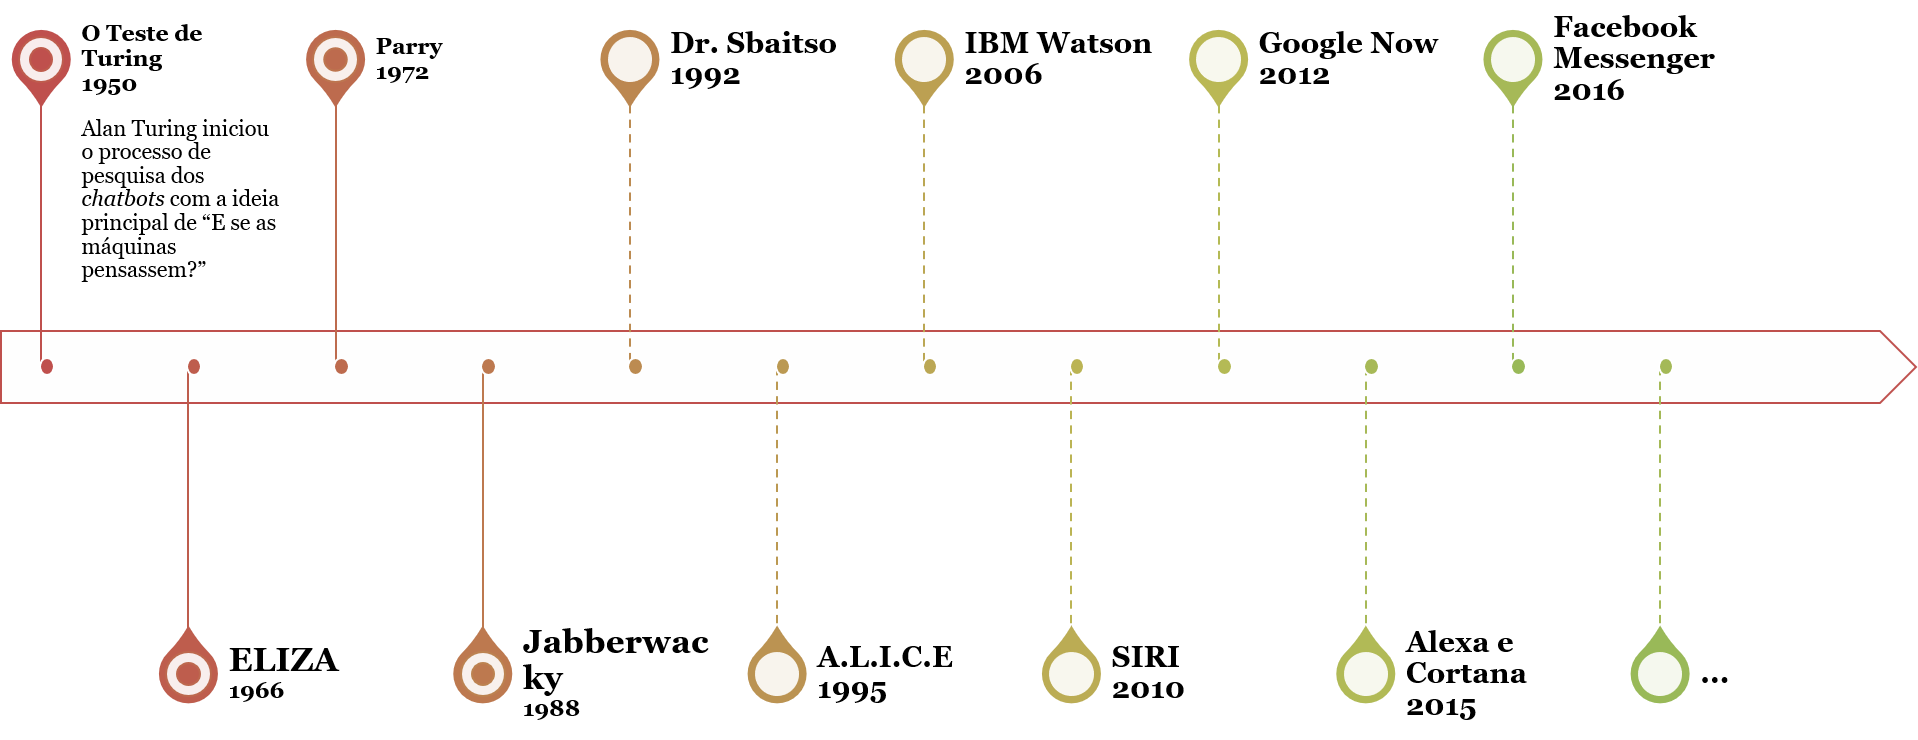
\includegraphics[width=15cm]{linhahistchatbots.png} % leia abaixo
\label{figura:Linha histórica dos chatbots}
\end{figure}

O termo IA foi criado pelos cientistas Newell, Simon, e J. C. Shaw, em 1956, deram início à tentativa do processamento simbólico, que seriam os sistemas que manipulavam símbolos em vez de serem somente baseados em números.
E então desde os anos 50, os diferentes estudos na área de IA consistem em criar e manter comportamentos inteligentes e com paridade humana nas máquinas, que se sintetizou em "Como fazer as máquinas compreenderem as coisas?"\cite{minsky}.

Com os estudos gerados a partir da tese de Turing, foram desenvolvidos esses \emph{chatbots}, para a simulação da interação humana, e o primeiro foi desenvolvido por Joseph Weizenbaum, em 1966. Tinha o intuito de simular uma terapeuta que fazia perguntas e interagia com o usuário de acordo com os termos inseridos durante toda a conversa, chamada Eliza.
Weizenbaum ficou surpreso como muitas pessoas não conseguiam distinguir Eliza de um psicólogo real. 
O principal método utilizado era o \emph{pattern matching}, ou procurar chaves, que seriam o sujeito e o verbo na frase, então transformando o “eu” em “você”, por exemplo, além de utilizar o resto da frase para construção da mensagem, trabalhando com a semântica da interação do usuário. \cite{weizenbaum-eliza}. Devido a essa simplicidade nos códigos, Eliza ainda não conseguia manter um diálogo prolongado com o usuário, e muitas vezes retornava o que ele dizia como forma de pergunta, isso fez com que mesmo sendo um avanço na tecnologia da época, ainda assim não passasse no teste de Turing, que será visto no próximo capítulo.

Com o passar dos anos, a partir da década de 70, novos robôs inteligentes foram sendo desenvolvidos, como por exemplo, Parry, em 1972, na Universidade de Stanford, simulando uma pessoa com esquizofrenia. 

Em 1988, foi lançado o Jabberwacky, desenvolvido para ser um robô de conversação que passasse no teste de Turing, com uma conversa bem-humorada, mas não cumpria com todos os requisitos para passar no mesmo. 
Em 1992, o \emph{chatbot} Dr. Sbaitso, feito para o MS DOS, funcionava de forma com que a interação fosse feita de forma falada, com a voz, ainda sendo totalmente inovador, a voz não se parecia com um humano e seus dados ainda eram bem limitados, parecido com a Eliza de Weizenbaum.

Já em 1995, foi desenvolvida a \emph{Artificial Linguistic Internet Computer Entity (ALICE)}, um dos softwares mais famosos na área de inteligência artificial e \emph{chatbots}. Foi programado em AIML e baseado em .XML, ALICE fornecia respostas pré-programadas de acordo com a interação do usuário e mesmo não passando no teste de Turing, ganhou alguns prêmios nessa área, hoje é um software de código aberto, que pode ser modificado e estudado por programadores do mundo todo.

Com o avanço do processamento de dados, da internet e da computação de um modo geral, a IBM lançou o seu chatbot, Watson, em 2006, os tipos de uso de aplicações cognitivas incluem entender emoções, interpretar textos e imagens, dar respostas, ouvir sons entre outros.\cite{ibm-watson}

O grande avanço da tecnologia trouxe em 2010 a Siri da \emph{Apple}, em 2012 o Google Now da \emph{Google}, em 2015 a Alexa da \emph{Amazon} e a Cortana da \emph{Microsoft}, que são considerados grandes \emph{chatbots} de assistência virtual usando linguagem natural para responder questões, fazer recomendações e ações utilizando os sistemas da internet para os usuários das plataformas que eles estão inseridos.


\subsection{Teste de Turing}
O teste de Turing, ou jogo da imitação, tem como objetivo analisar se o \emph{chatbot} consegue manter uma conversa computacional que seja praticamente imperceptível de que não seja humana.

O Turing aplicou esse teste considerando três pessoas, um interrogador, ou juiz, em uma sala separada, conversando com dois candidatos de sexos diferentes por meio de uma teleimpressora (aparelho telegráfico que permite a impressão da mensagem recebida em caracteres de imprensa, por meio de teclado semelhante ao da máquina de escrever; teleimpressor), para que a voz não fosse uma característica que interferisse na decisão final e que com base nas repostas, o interrogador conseguiria descobrir o sexo de cada um.

A pergunta “As máquinas podem pensar?” é substituída por “O que vai acontecer se a máquina se passar pela parte 'A' neste jogo”, o que traz à tona se as máquinas conseguem se passar por seres humanos em uma conversa, enganando então o interrogador ou o juiz da situação.\cite{Turing}

Nos dias atuais, segundo \textcite{LukaBradesko}, a forma que o teste é aplicado é com o observador, sendo o humano, que questiona ou dialoga com alguém através de um \emph{link} no computador. Esse alguém pode ser o \emph{chatbot}, e tem como objetivo fazer com que o observador acredite que é outro humano. Se o objetivo for alcançado, o \emph{chatbot} então passa no teste de Turing.


\section{Arquitetura e design de \emph{chatbots}}
\section{Arquitetura}
Segundo \textcite{Abdul-Kader2015}, o design e a arquitetura de um \emph{chatbot} podem ser dividida em três partes, são:

\begin{enumerate}

        \item \emph{Responder}: é a parte que desempenha as atividades entre o bot e o usuário.
        \item \emph{Classifier}: é a parte central, encontrada entre o \emph{Responder} (onde se recebe a entrada) e o \emph{Graphmaster}, e seu funcionamento tem como objetivo filtrar essa entrada, classificá em segmentos e a passagem pelos seus componentes lógicos, transferindo então a frase e/ou entrada para o \emph{Graphmaster}.
        \item \emph{Graphmaster}: é a parte que desempenha a função de construção da resposta, lidando então com as instruções das bases de dados e organizando os conteúdos para fazer a devolução da resposta de maneira com maior paridade e entendimento humano.
\end{enumerate}

As partes que constroem a arquitetura do \emph{chatbot} necessitam de alguns pontos principais que serão abordados nas próximas seções.

\subsection{Estratégias de comunicação}
\subsubsection{Conversão de fala para texto}
A fala é um dos mais poderosos meios de comunicação, e mais natural também. Segundo \textcite{Abdul-Kader2015}, a fala é amplamente aceita como o futuro da interação com aplicativos de computador e dispositivos móveis.
 
\textcite{wired-for-speech} mostram que aos \emph{chatbots} incorporarem o processamento de voz, serão então capazes de gerar uma interface sobre telefones e também rádios.
 
A conversão de voz em texto é chamada de \emph{Automatic Speech Recognition (ASR)} ou Reconhecimento Automático de Voz (RAV) e o objetivo é alcançar o reconhecimento de voz de um extenso vocabulário, independente de quem fala.

\textcite{wired-for-speech-2} mostram que a implementação e melhoria desse reconhecimento pode ser medida através de alguns fatores, tais como:

\begin{itemize}
	\item Tamanho do vocabulário: A variação de caracteres, letras maiúsculas e minúsculas, dígitos, e milhões de palavras em vários idiomas.
	\item Independência do locutor: capacidade de reconhecer locutores específicos, ou seja, gerar respostas específicas usando a identidade do locutor.
	\item Co-articulação: capacidade de processar um fluxo contínuo de palavras. Requer tokenização e segmentação adequadas do fluxo de entrada.
	\item Tratamento de ruído: capacidade de filtrar o que é a fala e o que é ruído, por exemplo, música de fundo, tráfego, etc.)
	\item Microfone: capacidade de processar a fala em variadas distâncias do microfone.
\end{itemize}

O processo ASR é dito então como não determinístico porque para cada tentativa de comunicar uma palavra, o som pode ser diferente por causa do ruído ambiente, estado emocional, distância do microfone, cansaço, entre outros fatores, mas pode ser modelado como um processo estocástico. Dado um som X, gera então o fonema mais provável, palavra, frase ou sentença de todas as palavras na língua.

\subsubsection{Processamento de linguagem natural}
Segundo \textcite{spoken-language-understan.}, o processamento de linguagem natural, conhecido também \emph{Natural Language Processing (NLP)}, tem como objetivo obter a saída do reconhecimento automático de voz e gerar uma representação estruturada do texto, conhecida como \emph{Spoken Language Understanding (SLU)} ou no caso de uma entrada de texto, \emph{Natural Language Understanding(NLU)}.

Empenha-se explorando formas de extrair semanticamente informações e significados escritos e falados para criar estruturas de dados gramaticais que podem ser processados pelo gerador de respostas.

Conforme \textcite{conversational-interface}, uma das formas de extrair um significado de uma linguagem natural é com o \emph{Dialogue Act (DA)}, ou ato de diálogo, atua reconhecendo a função das frases, se são sugestões, perguntas, comandos, entre outros. Então, após o reconhecimento dessa função, ela é classificada e um modelo estatístico de aprendizado de máquina é construído, usando uma série de recursos para classificar, como por exemplo, “por favor” retorna uma função de solicitação, “você é” retorna uma função de pergunta de resposta binária (sim/não), e informação sintática e semântica.

Segundo \textcite{da-recognition}, para iniciar o modelo de sistema de reconhecimento DA é necessário definir as principais funções, isso inclui escolher as classificações de uma forma que funcionem de uma forma generalizada para serem reutilizadas em outras frases, mas específicas o suficiente para continuar sendo relevantes para o texto alvo. Um conjunto de classificações que ganham destaque em \emph{chatbots} que utilizam DA são: \emph{Dialog Act Markup in Several Layers (DAMSL)}, que é  marcação do ato de dialogo em várias camadas, \emph{Switchboard SWBD-DAMSL}, gravador de reunião, \emph{VERBMOBIL} e \emph{Map-Task}.

\textcite{damsl} explicam que o esquema DAMSL classifica a frase em quatro dimensões, sendo elas:

\begin{itemize}
	\item 
	Status comunicativo: Classifica como não interpretável, abandonada ou fala interna.
	\item 
	Nível de informação: Classifica como tarefa, gerenciamento de tarefas, gerenciamento de comunicação ou outro.
	\item 
	Funções voltadas ao futuro: Codificam qualquer informação que afetará conversas e classificações futuras em oito subdimensões, sendo:
	\begin{itemize}
		\item Declaração: afirmar, reafirmar ou outro.
		\item Influenciar: opção aberta ou diretiva de ação.
		\item Solicitação de informações.
		\item Comprometer o orador a ações futuras: oferecer ou compromisso.
		\item Convencional abertura ou fechamento.
		\item Performativo explícito.
		\item Exclamação.
		\item Outros.
	\end{itemize}
	\item Funções voltadas ao passado: Codificam a relação entre o texto atual e o anterior em:
	\begin{itemize}
		\item Acordo.
		\item Entendimento.
		\item Resposta
		\item Relação de informação.
	\end{itemize}

\end{itemize}

\textcite{dasml-switchboard} afirmam que o \emph{Switchboard SWBD-DAMSL} é uma adaptação do DAMSL para automatização de conversas telefônicas. \textcite{shriberg-etal-2004-icsi}, afirmam que o gravador de reunião é semelhante ao \emph{Switchboard}, mas com classificações de 72 horas de reuniões, e lidando bem com rodeios e complicações típicas durante reuniões, como sobreposição de alto-falantes, frequência de abandono de comentários, interações e tomadas de voz. E o Map Task, segundo \textcite{map-task}, é uma hierarquia de níveis, onde o primeiro classifica as transações, o segundo são jogos conversacionais que classificam padrões como pares de perguntas e respostas, e o terceiro inclui 19 movimentos conversacionais.

A principal responsabilidade do reconhecimento de voz não é apenas entender a função das frases, mas também compreender o significado do próprio texto.
Para extrair o significado do texto, temos que converter os textos não estruturados, sendo eles saídas do ASR ou o texto escrito como entrada, em objetos de dados gramaticais, que serão processados pelo DA.\cite{conversational-interface}

\textcite{conversational-interface} explicam que o primeiro passo neste processo de extração é quebrar uma frase em \emph{tokens} que representam cada parte do seu componente, sendo palavras, dígitos, sinais de pontuação ou outros. Essa transformação para \emph{tokens} pode ser mais complexa devido a entradas ambíguas ou mal formadas, como contradições, abreviações e pontuações, que para desenvolverem uma série de estruturas de dados diferentes para serem processadas pelo gerenciador de diálogos podem ser analisados utilizando as seguintes técnicas:

\begin{itemize}
	\item Amontoado de palavras: Tem como objetivo formar um modelo de espaço vetorial, para isso são ignoradas a estrutura, a ordem e a sintaxe das frases, contando o número de ocorrências de cada palavra. Com isso as palavras de parada, como artigos, são removidas, e as variantes morfológicas passam pelo processo de lematização onde são armazenadas como uma instância do lema básico. Possui uma abordagem simples, por ignorar a sintaxe das frases e por esse motivo não é tão precisa para problemas mais complexos.
	\item \emph{Latent Semantic Analysis (LSA)} ou análise semântica latente: Tem uma atuação parecida com o amontoado de palavras. Conceitos são a unidade básica de comparação analisada a partir da frase. Depois, as palavras que se repetem são agrupadas. É criada então, uma matriz onde cada linha representa uma palavra, cada coluna um documento e o valor de cada célula é a frequência da palavra no documento. É calculada a distância entre o vetor que representa cada texto e documento, usando a decomposição de valor singular para reduzir a dimensionalidade da matriz e determinar o documento mais próximo.
	\item Expressões regulares: Frases podem ser tratadas como expressões regulares e podem ser padronizadas com os documentos no banco de dados existente na base de conhecimento do \emph{bot}. Por exemplo, um desses documentos lida com o caso em que o usuário insere a frase: "meu nome é *". “*” É o caractere coringa e indica que essa expressão regular deve ser acionada sempre que o \emph{bot} ouvir ou ler a frase “meu nome é” seguida por qualquer coisa. Se o usuário disser “meu nome é Jack”, essa frase será analisada em várias expressões regulares, incluindo “meu nome é *” e acionará a recuperação desse documento. 
	\item Marcações de partes do texto: Essa marcação classifica cada palavra no texto de entrada de acordo com sua classe gramatical, podendo ser substantivo, verbo, adjetivo e outros. Essas classificações podem ser baseadas em regras criadas manualmente para especificar a classe gramatical de palavras ambíguas de acordo com o contexto da frase, também podem ser criadas usando modelos estocásticos que treinam em frases marcadas com a parte correta do texto. No gerenciador de diálogos, a marcação de parte do texto pode ser usada para armazenar informações relevantes no histórico de diálogos. E também é usado na geração de respostas para indicar o tipo de objeto da resposta desejada. 
	\item Reconhecimento de Entidades Nomeadas (REN): Nesse caso, o nome de pessoas, lugares, grupos e locais são extraídos e classificados de acordo. Os pares de nomes podem ser armazenados pelo gerenciador de diálogos no histórico para acompanhar o contexto da conversa. A extração de relação vai um passo adiante para relações de identidade (por exemplo, "quem fez o quê a quem") e classifica cada palavra nestas frases.
	\item Rotulagem de função semântica: Nesse processo, o predicado é rotulado primeiro, logo após vem seus argumentos. Classificadores proeminentes para rotulagem de função semântica foram treinados no \emph{FrameNet} e \emph{PropBank}, bancos de dados com frases já classificadas com suas funções semânticas. Esses pares de palavras-funções semânticas podem ser armazenados pelo gerenciador de diálogos no histórico de diálogos para manter o controle do contexto.
	\item Criação de estrutura de dados gramaticais: Frases e enunciados podem ser armazenados de forma estruturada em formalismos gramaticais, como gramáticas livres de contexto, que são estruturas de dados semelhantes a árvores que representam sentenças contendo frases nominais e verbais, cada uma delas contendo substantivos, verbos, sujeitos e outras construções gramaticais, e gramáticas de dependência que por outro lado, focam nas relações entre as palavras. 
\end{itemize}


\subsubsection{Gerador de resposta}
De acordo com \textcite{response-generator}, o gerador de respostas é o componente central da arquitetura de um \emph{chatbot}. Recebendo uma representação estruturada do texto falado e devolvendo uma resposta para entregar ao usuário, que em seguida também passa a ser guardado no gerenciador de diálogo.

Para a tomada de decisão sobre a resposta a ser dada, existem três componentes importantes:
\begin{itemize}
	\item Uma base de conhecimento, ou banco de dados, que irá analisar de acordo com o que foi implementado.
	\item Um histórico de dados de diálogos, modelos mais complexos de \emph{chatbots} possuem a capacidade de armazenamento do histórico.
	\item Uma fonte de dados externa, ou a "inteligência do senso comum” que possibilita o \emph{bot} a fazer pesquisas em sites de busca para ser alimentado.
\end{itemize}

Modelos baseados em regras têm como principal base de conhecimento os documentos que possuem um <padrão> e um <modelo>. Assim que o \emph{chatbot} recebe uma entrada que se encaixa no <padrão>, faz com que retorne o modelo correspondente como saída.

\textcite{yan-etal-2016-docchat} trazem a especificação desses pares serem feitas a mão como um problema, e passam o conceito do modelo baseado em recuperação de dados, trabalhando com <status> e <resposta>, em vez de <padrão> e <modelo>. Então, ele recebe uma entrada e procura no histórico os pares de <status> e <resposta> correspondente. 

\subsubsection{Base de conhecimento}
A base de conhecimento de um \emph{chatbot} é a principal vertente de sua inteligência. Todos os dados que ele recebe por meio dessas bases são utilizados para a construção dos modelos para a devolutiva correta a entrada do usuário.

Essas bases de dados podem ser coletadas de várias formas, e esses dados podem ser armazenados, treinados para utilização de inteligência artificial para serem classificados como dados que podem ser devolvidos ao usuário com entendimento como interação humana, e podem ser coletados através de:

\begin{itemize}
	\item Fóruns de discussão \emph{online}: \textcite{oline-foruns-database} geraram uma base de conhecimento que busca em fóruns \emph{online} maneiras de respostas baseadas em \emph{<input><response>}. Tendo benefícios como a quantidade de tópicos e assuntos diferentes abordados nesses fóruns com diferentes respostas ou soluções para a mesma pergunta. Mas como desvantagem traz a não garantia da qualidade das respostas, tendo em vista que são publicadas por vários usuários, tendo eles conhecimento ou não sobre o assunto, podendo também trazer respostas curtas e não definidas. Também podem trazer erros de comunicação, considerando que os fóruns são baseados em \emph{threads} de resposta, então aquela <response> pode não corresponder exatamente aquele \emph{<input>}. Para resolver isso, eles desenvolveram uma forma de tratar e treinar uma Máquina de Vetor Classificador (MVC) de forma com que ela identifique as respostas e perguntas diretamente da raiz, a \emph{thread} que elas pertencem e a forma com que são usadas as palavras-chave. Depois dessa classificação pela MVC, são aplicados filtros para remover respostas que utilizam palavras obscenas, ou com respostas pessoais do achismo (por exemplo, “meu”, “opinião”) e respostas que foram classificadas pela MVC como fora da \emph{thread}. Devolvendo então o par \emph{<thread title><response>} para treinar o \emph{bot} dessa forma.

	\item \emph{Artificial Intelligence Markup Language (AIML)}: \textcite{AIML} explicam que o AIML funciona como forma de simplificar o modelo de diálogo, trabalhando com a definição da classe objeto que é responsável para fazer o molde dos padrões de conversa, responde de acordo com a conexão entre as questões previamente implantadas localizadas nos arquivos AIML definidos. Também possui suas vantagens e desvantagens, entre as vantagens estão a fácil implementação e aprendizado, o modo simples do sistema de diálogo o deixando intuitivo e o uso de XML representando uma forma de leitura para o computador, e entre suas desvantagem está o conhecimento fornecido pelos arquivos, por não existir extensões possível para o AIML Original e precisar sempre de atualização manual para implantação de novas perguntas e respostas, pode-se trabalhar com o AIML 2.0 acessando recursos externos com comandos para o Assistente Virtual de respostas.
	\item RiveScript: Funciona como o AIML, só que com algumas funcionalidades a mais, como o uso simplificado de expressões regulares de gatilhos de entrada de usuários, e pode ter integração com mecanismos ou sites de pesquisa para respostas dinâmicas.
\end{itemize} 

\subsubsection{Gerenciamento de diálogo}
O gerenciamento do diálogo funciona para transformar a resposta em uma forma mais parecida com a forma humana de responder, podendo utilizar estratégias de comunicação.

Dentre essas estratégias temos os truques de linguagem que são utilizados em caso de baixa probabilidade de resposta apropriada, \textcite{dialogue-manag.} mostram que isso pode fazer com que o \emph{bot} pode continuar a conversa e responda como: uma mudança de tópico, ou seja, propondo outros tópicos para ter novos dados ou melhor forma de responder ao usuário, pode também fazer uma pergunta aberta, que seria além de dizer que não sabe responder especificamente o que o usuário disse, faz uma pergunta em troca, para assim manter a conversa, pode também pedir ao usuário que diga mais informações sobre o que ele deseja, então além de continuar a conversa ainda tem chances de fazer a devolutiva de uma resposta mais apropriada ao usuário.

Uma interface que traz uma fluidez na conversa com a proximidade humana traz alguns conceitos de design que são importantes como o modo de transformar a entrada do usuário em uma entrada com mais clareza se tiver duplo sentido, habilidade de eliminar restrições para continuar a conversa com outra pergunta se necessário, confirmar detalhes  de tarefas que o \emph{bot} deve tomar para decisões importantes e perguntar detalhes necessários que aparentemente o usuário se esqueceu de informar.

%Este modelo vem com o ambiente \texttt{quadro} e impressão de Lista de quadros configurados por padrão. Verifique um exemplo de utilização:

%\begin{quadro}[htb]
%\caption{\label{quadro_exemplo}Exemplo de quadro}
%\begin{tabular}{|c|c|c|c|}
%	\hline
%	\textbf{Pessoa} & \textbf{Idade} & \textbf{Peso} & \textbf{Altura} \\ \hline
%	Marcos & 26    & 68   & 178    \\ \hline
%	Ivone  & 22    & 57   & 162    \\ \hline
%	...    & ...   & ...  & ...    \\ \hline
%	Sueli  & 40    & 65   & 153    \\ \hline
%\end{tabular}
%\fonte{Autor.}
%\end{quadro}

%Este parágrafo apresenta como referenciar o quadro no texto, requisito
%obrigatório da ABNT. 
%Primeira opção, utilizando \texttt{autoref}: Ver o \autoref{quadro_exemplo}. 
%Segunda opção, utilizando  \texttt{ref}: Ver o Quadro \ref{quadro_exemplo}.

% ----------------------------------------------------------
% PARTE
% ----------------------------------------------------------
\chapter{Desenvolvimento}
% ----------------------------------------------------------

Este capítulo apresenta uma descrição sobre a arquitetura e tecnologias escolhidas para o desenvolvimento de um \emph{chatbot}. O público-alvo serão os alunos do curso de Ciência da Computação do Centro Universitário Senac - Santo Amaro, com o objetivo de tirar dúvidas e agilizar a comunicação entre a secretaria/o coordenador e os mesmos.


\section{Metodologia}

A fala é amplamente aceita como o futuro da interação com assistentes eletrônicos conforme estabelecido na seção de conversão de fala para texto, porém, com o intuito de tornar o escopo do projeto mais administrável, optou-se pela interação por texto. Desta forma, o processamento de linguagem natural será realizado por um \emph{software} que baseia-se na \emph{NLU (Natural Language Understanding)}.

As seguintes tecnologias serão utilizadas para atender a arquitetura em três partes, apresentadas no capítulo 2.3:

\begin{figure}[h]
\centering % para centralizarmos a figura
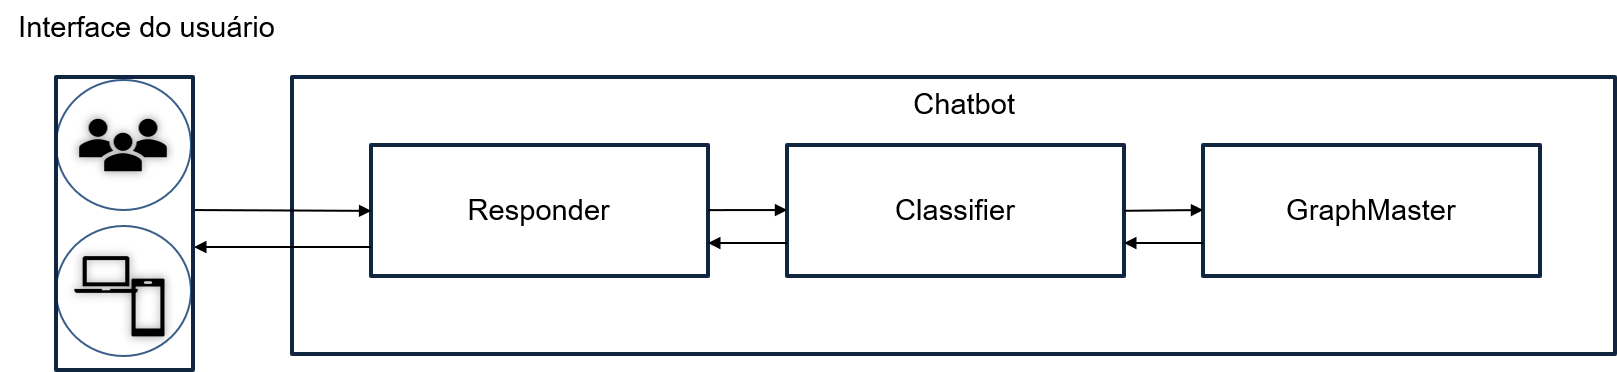
\includegraphics[width=15cm]{arquiturachatbot1.png} % leia abaixo
\label{figura:Linha histórica dos chatbots}
\end{figure}

\begin{enumerate}
\item \emph{Responder}: composto por uma caixa de digitação e painel de visualização desenvolvidos em Python com o auxílio da biblioteca tkinter; esta é uma ponte em Python para criação de telas interativas através do \emph{toolkit} Tk. O \emph{Responder} é responsável por transmitir para e receber textos do \emph{Classifier}.
\item \emph{Classifier}: conforme citado anteriormente no capítulo em questão, é a secção responsável pelo processamento da entrada e posterior transferência para a última parte, o \emph{Graphmaster}. Neste módulo encaixa-se o software \emph{NLU}. Será utilizado o \emph{Natural Language Processing Toolkit (NLTK)}, um \emph{plugin} gratuito para Python mencionado também por \textcite{Abdul-Kader2015} como uma plataforma amplamente utilizada.
\item \emph{Graphmaster}: o cérebro do \emph{software} onde são produzidas as respostas para a entrada pré-processada recebida do \emph{Classifier}. O treinamento será efetuado com auxílio de \emph{deep learning} através da biblioteca Keras; esta permite um desenvolvimento de forma \emph{‘fail fast, fail early’}.
\end{enumerate}

A base de dados será armazenada em nuvem na plataforma Azure e receberá os dados primeiramente através de um formulário, previamente alinhado com o coordenador do curso, enviado para os alunos de diferentes semestres do curso de Ciência da Computação com perguntas como:
\begin{enumerate}
\item Quais foram as principais dúvidas que você teve ao entrar no curso? (Campo aberto)
\item Quais dúvidas você tem com frequência para perguntar ao coordenador? (Campo aberto)

\item Ao entrar no curso ou até mesmo no dia a dia, você teve alguma das dúvidas para esclarecer com o coordenador ou com os professores do seu curso? Selecione com base na frequência deste questionamento:
\begin{itemize}
\item “Eu preciso saber matemática?"
\item “Qual nível de inglês eu preciso ter para conseguir me formar?”
\item “Quais matérias eu terei nesse semestre?”
\item “Quantas matérias de cálculo eu terei durante o curso?”
\item “Quais matérias eu terei de eletivas para esse semestre?”
\item “Quantas DPs eu posso pegar para conseguir passar para o próximo semestre?”
\item “Quais professores irão me dar aula?”
\item “Durante o curso, quantas aulas eu terei?”
\item “Qual horário da minha aula hoje?”
\item “Quais as instalações do campus?”
\item“O campus possui instalação X?”
\end{itemize}

\item Em uma escala de 0 a 5, o quão importante você considera os seguintes requisitos para as respostas de suas dúvidas?
\begin{itemize}
\item 0 - 5 : Agilidade
\item 0 - 5 : Interação humana
\item 0 - 5 : Interação por voz
\item 0 - 5 : Modo de resposta formal
\item 0 - 5 : Modo de resposta informal
\end{itemize}

\end{enumerate}

O objetivo final é oferecer o serviço permanentemente para os alunos. Porém, somente durante o desenvolvimento será identificada a real complexidade do projeto e, ao término, a usabilidade do produto final. Desta forma o software será hospedado localmente até a apresentação final. Caso o experimento seja bem-sucedido e viável para aplicação real, considera-se a implementação no \emph{website} da instituição, se tal laurel for concedido aos alunos deste trabalho. As ferramentas mencionadas foram escolhidas de tal forma a propiciar esta transição de forma fluida, como o banco de dados em nuvem e a biblioteca Keras, que permite a geração de modelos em \emph{Javascript} que executam diretamente no navegador.

% ---
% Capitulo de desenvolvimento
% ---
%\chapter{Método utilizado}
%\chapter{Construção do \emph{chatbot}}
%\chapter{Testes}
%\chapter{Avaliações}


% ----------------------------------------------------------
% PARTE
% ----------------------------------------------------------
%\part{Conclusão}
% ----------------------------------------------------------


% ----------------------------------------------------------
% Finaliza a parte no bookmark do PDF
% para que se inicie o bookmark na raiz
% e adiciona espaço de parte no Sumário
% ----------------------------------------------------------
\phantompart

% ----------------------------------------------------------
% ELEMENTOS PÓS-TEXTUAIS
% ----------------------------------------------------------
\postextual
% ----------------------------------------------------------

% ----------------------------------------------------------
% Referências bibliográficas
% ----------------------------------------------------------
%\bibliography{abntex2-modelo-references}

\printbibliography[title = Referências]
% ----------------------------------------------------------
% Glossário
% ----------------------------------------------------------
%
% Consulte o manual da classe abntex2 para orientações sobre o glossário.
%
%\glossary

% ----------------------------------------------------------
% Apêndices
% ----------------------------------------------------------

% ---
% Inicia os apêndices
% ---
%\begin{apendicesenv}
%
%% Imprime uma página indicando o início dos apêndices
%\partapendices
%
%% ----------------------------------------------------------
%\chapter{Quisque libero justo}
%% ----------------------------------------------------------
%
%\lipsum[50]
%
%% ----------------------------------------------------------
%\chapter{Nullam elementum urna vel imperdiet sodales elit ipsum pharetra ligula
%ac pretium ante justo a nulla curabitur tristique arcu eu metus}
%% ----------------------------------------------------------
%\lipsum[55-57]
%
%\end{apendicesenv}
%% ---
%
%
%% ----------------------------------------------------------
%% Anexos
%% ----------------------------------------------------------
%
%% ---
%% Inicia os anexos
%% ---
%\begin{anexosenv}
%
%% Imprime uma página indicando o início dos anexos
%\partanexos
%
%% ---
%\chapter{Morbi ultrices rutrum lorem.}
%% ---
%\lipsum[30]
%
%% ---
%\chapter{Cras non urna sed feugiat cum sociis natoque penatibus et magnis dis
%parturient montes nascetur ridiculus mus}
%% ---
%
%\lipsum[31]
%
%% ---
%\chapter{Fusce facilisis lacinia dui}
%% ---
%
%\lipsum[32]
%
%\end{anexosenv}

%---------------------------------------------------------------------
% INDICE REMISSIVO
%---------------------------------------------------------------------
\phantompart
\printindex
%---------------------------------------------------------------------

\end{document}